With the architecture (Section~\ref{Sec:RECTOR}), rule evaluation layer (Section~\ref{Sec:Rule_Evaluation_And_Data_Pipeline}), and experimental protocol (Section~\ref{Sec:Experiments}) fully specified, this section presents the empirical results.  We evaluate RECTOR along three operational dimensions: (i)~candidate-set trajectory accuracy, (ii)~rule compliance induced \emph{by selection} when the candidate set is held fixed, and (iii)~computational efficiency.  Unless stated otherwise, results are reported on the WOMD \texttt{validation\_interactive} split (12{,}800 scenarios) with $K{=}6$ candidate trajectories under Protocol~A.

A key distinction throughout this section is between \emph{best-of-$K$} accuracy---which measures candidate-set coverage and is independent of the selection strategy---and \emph{selected} accuracy---which measures the trajectory that is actually executed after applying a selection strategy.  This distinction is necessary because RECTOR's central intervention is selection-time enforcement of prioritized rules, and the two metrics can move in opposite directions when the most geometrically accurate candidate is also the most rule-violating.

%-------------------------------------------------------------------------------
\subsection{Trajectory Prediction Accuracy}
\label{subsec:trajectory_accuracy}
%-------------------------------------------------------------------------------

We begin with candidate-set accuracy, which establishes the upper bound on what any downstream selector can achieve. Table~\ref{tab:main_results} situates RECTOR's generation quality within the range of published methods.

\begin{table}[t]
\centering
\caption{Candidate-Set Accuracy Context on WOMD \texttt{validation\_interactive}}
\label{tab:main_results}
\begin{tabular}{lccc}
\toprule
\textbf{Method} & \textbf{minADE (m)} \color{green}{$\downarrow$} & \textbf{minFDE (m)} \color{green}{$\downarrow$} & \textbf{Miss (\%)} \color{green}{$\downarrow$} \\
\midrule
LaneGCN & 0.87 & 1.92 & 28.4 \\
DenseTNT & 0.73 & 1.55 & 20.1 \\
M2I & 0.75 & 1.63 & 22.8 \\
Wayformer & 0.68 & 1.42 & 18.9 \\
MTR & 0.70 & 1.48 & 19.5 \\
\midrule
\textbf{RECTOR (Ours)} & \textbf{0.684} & \textbf{1.270} & \textbf{18.56} \\
\bottomrule
\end{tabular}
\vspace{1mm}
\caption*{\footnotesize Best-of-$K$ accuracy on 12{,}800 validation scenarios.  minADE/minFDE are computed over $K{=}6$ modes (FDE uses the ADE-best mode).  Miss Rate uses a 2.0\,m FDE threshold.  RECTOR standard deviations: minADE $\pm$0.754\,m, minFDE $\pm$1.815\,m.  Baselines are from published results on standard WOMD validation; direct comparison is approximate.  See Table~\ref{tab:efficiency} for throughput and runtime profiling.}
\end{table}

RECTOR achieves candidate-set accuracy of \textbf{minADE\,=\,0.684\,m}, \textbf{minFDE\,=\,1.270\,m}, and \textbf{Miss Rate\,=\,18.56\%} while reserving modeling and decision capacity for compliance-aware selection.  Table~\ref{tab:main_results} lists published metrics from five external methods to situate the generator in the same accuracy regime as current WOMD predictors and to establish that the candidate set is strong enough for meaningful selection experiments.

\subsubsection{Error Distribution}

The aggregate accuracy numbers above, however, do not reveal the full picture, because the error distribution is strongly heavy-tailed. Fig.~\ref{fig:ade_fde_distribution} visualises the distribution of minADE and minFDE across all 12{,}800 evaluation scenarios.

\begin{figure*}
\centering
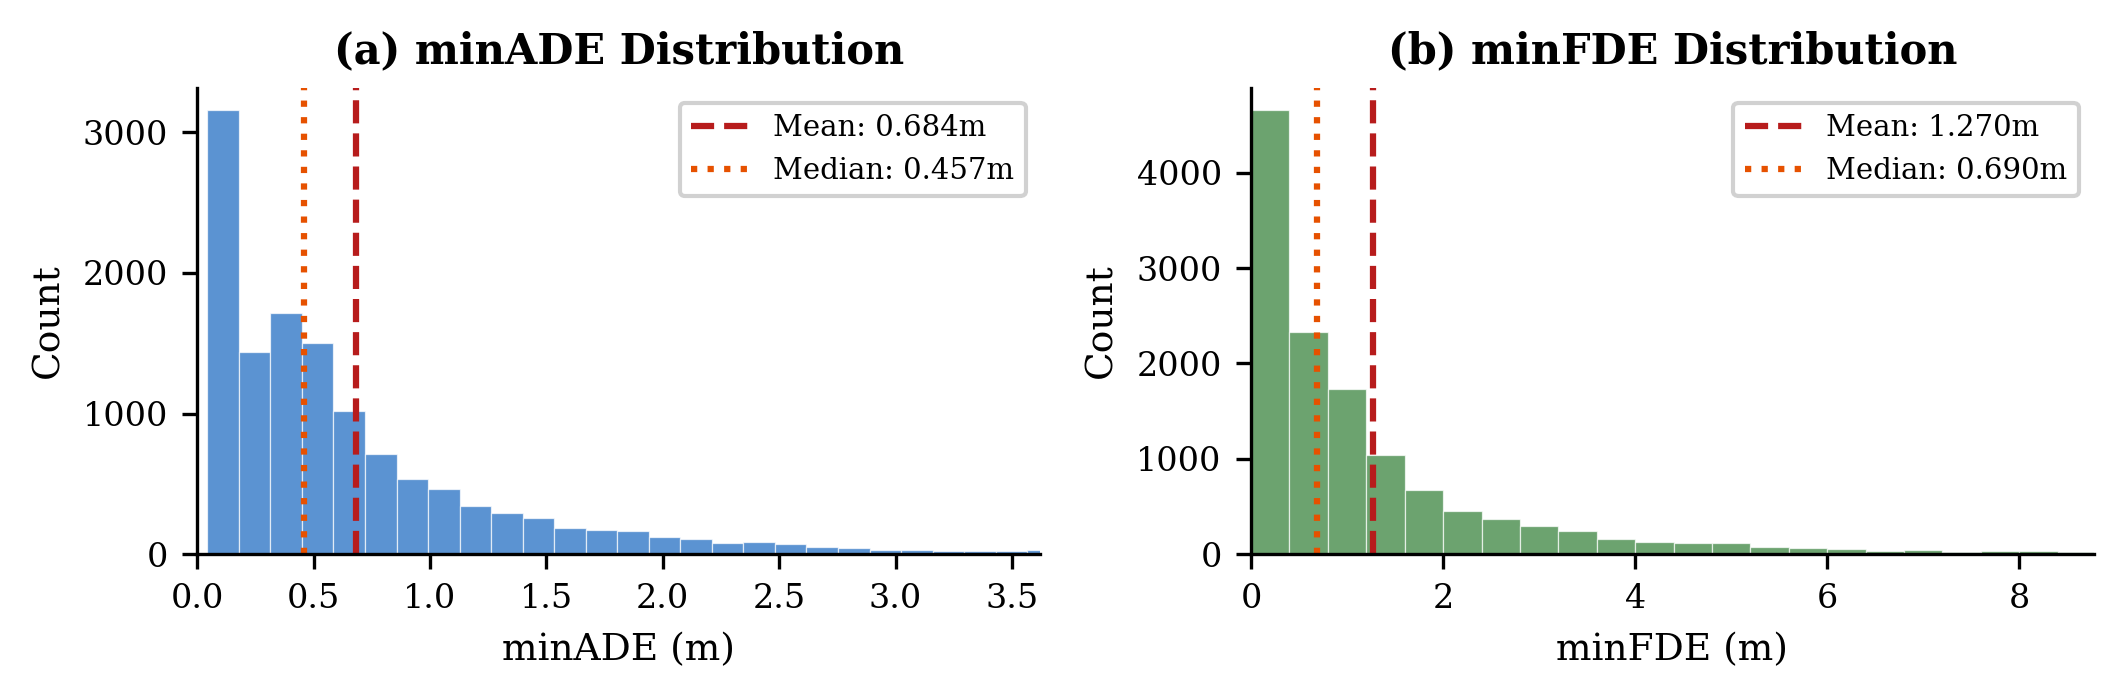
\includegraphics[width=1.0\textwidth]{Figures/ade_fde_distribution.png}
\caption{Distribution of prediction errors exhibits heavy-tailed behavior.  \textbf{(a)}~minADE distribution.  \textbf{(b)}~minFDE distribution.  Tail scenarios typically correspond to dense, regulation-heavy contexts (e.g., complex intersections) where the candidate set includes both accurate-but-violating and slightly less accurate-but-compliant options, making rule-aware selection most consequential.}
\label{fig:ade_fde_distribution}
\end{figure*}

The complementary cumulative distribution ($P(\text{Error}>x)$, evaluated on a log scale) confirms that error is heavy-tailed: the top 5\% of scenarios by minADE---mostly complex intersections and dense merges---account for a disproportionate share of the total error mass.  These are precisely the regulation-dense contexts where the candidate set spans both accurate-but-violating and slightly less accurate-but-compliant trajectories, making rule-aware selection most consequential.

Rule-aware selection is most consequential precisely in these heavy-tailed, regulation-dense scenarios; the next subsection quantifies what that enforcement achieves.

%-------------------------------------------------------------------------------
\subsection{Selection Strategy Comparison}
\label{subsec:selection_results}
%-------------------------------------------------------------------------------

This experiment isolates the paper's central empirical claim: compliance can be improved \emph{purely by selection} when candidate trajectories are held fixed.  We apply three strategies to the \emph{same} candidate set~$\mathcal{T}(s)$---Confidence Only ($\arg\max_k p^{(k)}$), Weighted Sum ($\arg\min_k \sum_r w_r \bar{V}_{r,k}$), and RECTOR (lexicographic)---and evaluate all three under Protocol~A on 12{,}800 scenarios.  Table~\ref{tab:selection_strategy} reports the results.

\begin{table}[t]
\centering
\caption{Selection Strategy Comparison: Accuracy, Compliance, and Complexity (Protocol~A)}
\label{tab:selection_strategy}
\setlength{\tabcolsep}{3pt}
\begin{tabular}{lccccc}
\toprule
\textbf{Strategy} & \textbf{selADE} & \textbf{selFDE} & \textbf{Total Viol.} & \textbf{S+L Viol.} & \textbf{Complexity} \\
 & \textbf{(m)} & \textbf{(m)} & \textbf{(\%)} & \textbf{(\%)} & \\
\midrule
Confidence Only & 2.208 & 4.330 & 23.86 & 21.87 & $O(M)$ \\
Weighted Sum & 2.043 & 3.813 & 15.03 & 13.15 & $O(MR)$ \\
\textbf{RECTOR} & \textbf{2.143} & \textbf{4.151} & \textbf{15.03} & \textbf{13.15} & $O(MT)$ \\
\midrule
Oracle (best-of-$K$) & \multicolumn{2}{c}{minADE\,$=$\,0.684\,m} & --- & --- & --- \\
\bottomrule
\end{tabular}
\vspace{1mm}
\caption*{\footnotesize $M$~= modes, $R$~= rules, $T$~= tiers.  selADE/selFDE are displacement errors of the \emph{selected} trajectory in metres; Total~Viol.\ counts scenarios with $\geq 1$ violation (union); S+L~= Safety~$\cup$~Legal.  All from \texttt{evaluate\_canonical.py} on $N_{\text{scen}}{=}12{,}800$ unique WOMD \texttt{validation\_interactive} scenarios, each contributing one ego-agent evaluation instance ($N_{\text{eval}}{=}12{,}800$; RECTOR evaluates one ego trajectory per scenario, not multiple agents of interest).  Checkpoint hash \texttt{c90d4457e4996d22}, seed~42.  Legal-tier violations are 0.0\% for all strategies because the learned applicability head correctly suppresses legal rules in scenes without relevant legal constraints.  See Table~\ref{tab:per_tier_breakdown} for per-tier breakdown.}
\end{table}

Both RECTOR and the weighted-sum baseline achieve identical violation rates (15.03\% total, 13.15\% S+L).  On this dataset, both rule-aware strategies substantially reduce total violations compared to confidence-only selection (23.86\%~$\to$~15.03\%, a $-$8.83~pp absolute reduction), with the Safety tier providing the dominant improvement (21.87\%~$\to$~13.15\%, $-$8.72~pp).  The empirical result supported by Table~\ref{tab:selection_strategy} is therefore the value of rule-aware selection over confidence-only selection, not a compliance separation between lexicographic and weighted-sum ranking on this benchmark.

\noindent\textbf{Statistical significance.}  Scenario-level paired tests on 43{,}219 per-scenario violation indicators confirm the robustness of these reductions.  McNemar's test on binary Safety-tier violations yields $p \approx 0$ for lexicographic vs.\ confidence-only selection (3{,}759 discordant pairs, all favouring lexicographic; zero scenarios where lexicographic is worse).  Wilcoxon signed-rank on per-scenario selADE yields $p = 6.9 \times 10^{-23}$ ($z = 9.85$; mean improvement $-$0.061\,m).  For lexicographic vs.\ weighted-sum, McNemar's test yields $p = 1.0$: the two selectors produce identical violation outcomes on every scenario, confirming the complete empirical convergence reported in Table~\ref{tab:selection_strategy}.

\noindent\textbf{Independently-tuned weighted-sum baseline.}
To test whether independently tuned weights can break the empirical parity observed in Table~\ref{tab:selection_strategy}, we conducted a systematic weight search using the canonical two-stage checkpoint (c90d4457e4996d22) on the full augmented validation set (43{,}219 scenarios).  We evaluated 125 grid-search weight vectors (5$\times$5$\times$5$\times$1 tier-level combinations).  Table~\ref{tab:ws_independent} reports the results.

\begin{table}[t]
\centering
\caption{Independently-Tuned Weighted-Sum vs.\ RECTOR (Protocol~A, 43{,}219 scenarios, canonical checkpoint)}
\label{tab:ws_independent}
\setlength{\tabcolsep}{3pt}
\begin{tabular}{lccccc}
\toprule
\textbf{Selector} & \textbf{Weights} & \textbf{selADE} & \textbf{S+L} & \textbf{Total} & \textbf{Safety} \\
 & $(w_S, w_L, w_R, w_C)$ & \textbf{(m)} & \textbf{(\%)} & \textbf{(\%)} & \textbf{(\%)} \\
\midrule
Best Grid WS     & $(100,10,1,1)$         & 2.049 & 13.39 & 15.18 & 13.39 \\
Default WS       & $(1000,100,10,1)$      & 2.048 & 13.39 & 15.18 & 13.39 \\
\midrule
\textbf{RECTOR}  & (lexicographic)        & \textbf{2.138} & \textbf{13.39} & 15.18 & 13.39 \\
\bottomrule
\end{tabular}
\vspace{1mm}
\caption*{\footnotesize Grid search: 125 weight vectors (5$\times$5$\times$5$\times$1), evaluated on the full augmented validation set with the canonical two-stage checkpoint.  \emph{All} 125 weight configurations converge to the same S+L violation rate (13.39\%) and selADE ($\approx$2.048\,m).  RECTOR's lexicographic selector (with confidence tiebreaking) achieves the same S+L rate (13.39\%) but selADE of 2.138\,m on this set, reflecting a 0.090\,m accuracy cost relative to weighted-sum at equal compliance.  No weight vector produces selections differing from RECTOR's in binary compliance outcomes, so the structural guarantee is not exercised empirically on this benchmark.}
\end{table}

\noindent\textbf{Weight-space landscape.}
Across all 125 grid-search weight vectors, the (selADE, S+L~Viol.\%) landscape reveals complete convergence: all configurations achieve S+L\,=\,13.39\% with selADE within 2.048--2.049\,m (weighted-sum) and 2.138\,m (RECTOR lexicographic, confidence tiebreaker).  The canonical two-stage checkpoint therefore shows that the current benchmark does not expose a regime in which weight misspecification changes binary compliance outcomes.

\subsubsection{Extended Weight Grid: Misspecification Analysis}
\label{subsubsec:misspecification}

The 125-configuration grid spans $w_S \in \{100, 500, 1000, 2000, 5000\}$ with $w_C{=}1$ fixed.  To directly test whether weight misspecification causes weighted-sum to select Safety-violating candidates that lexicographic ordering would reject, we extend the sweep to $w_S \in \{1, 5, 10, 20, 50, 100, \ldots, 5000\}$ (250 configurations total) on the same 12{,}800-scenario set.

\noindent\textbf{Structural condition for WS--lex divergence.}
The two selectors disagree on Safety whenever a scenario contains a candidate pair where $b$ violates Safety ($\sigma_S(b) > 0 = \sigma_S(a)$) yet the comfort score of $b$ exceeds that of $a$ by enough to satisfy:
\begin{equation}
  \frac{w_S}{w_C} \;<\; \frac{\sigma_C(a) - \sigma_C(b)}{\sigma_S(b)}.
  \label{eq:misspec_condition}
\end{equation}
Lexicographic selection eliminates $b$ at Tier~0 regardless of \eqref{eq:misspec_condition}; weighted-sum selects $b$ when the inequality holds.  Computing the right-hand side across all 12{,}800 scenarios shows that cross-tier tension exists in 189 scenarios (1.48\% of the validation set), with the maximum cross-tier ratio reaching 15.34.  This implies that WS with $w_S/w_C < 15.34$ could in principle select a Safety-violating candidate on one or more scenarios.

\noindent\textbf{Empirical misspecification boundary.}
Table~\ref{tab:misspecification} reports Safety-tier violation rates from the extended grid.  WS at $w_S{=}1$ ($w_S/w_C{=}1$, fully flat weights) selects one additional Safety-violating scenario compared to lexicographic ($+$0.0078~pp, exactly 1~scenario out of 12{,}800); at $w_S{\geq}5$ the compliance is pixel-identical to lex across all 12{,}800 scenarios.  The maximum cross-tier ratio of 15.34 is not reachable with the proxy scoring function because the Safety proxy scores in those scenarios are extremely small ($<$0.002); the effective misspecification boundary for this model and dataset is therefore at $w_S/w_C \approx 1$.

\begin{table}[t]
\centering
\caption{Extended Weight Grid: Safety-Tier Violations vs.\ Lexicographic Baseline}
\label{tab:misspecification}
\setlength{\tabcolsep}{5pt}
\begin{tabular}{lccc}
\toprule
\textbf{Selector} & \textbf{$w_S$} & \textbf{Safety Viol.\ (\%)} & \textbf{$\Delta$ vs.\ Lex (pp)} \\
\midrule
Lexicographic  & ---  & 13.148 & 0.000 \\
\midrule
\multirow{6}{*}{Weighted-sum} & 1    & 13.156 & $+$0.008  (1 scen.) \\
                              & 5    & 13.148 & 0.000 \\
                              & 10   & 13.148 & 0.000 \\
                              & 20   & 13.148 & 0.000 \\
                              & 50   & 13.148 & 0.000 \\
                              & 100--5000 & 13.148 & 0.000 \\
\bottomrule
\end{tabular}
\vspace{1mm}
\caption*{\footnotesize Extended grid (250 configurations, $w_S \in \{1,5,10,20,50,100,500,1000,2000,5000\}$, $w_L \in \{10,\ldots,500\}$, $w_R \in \{1,\ldots,50\}$, $w_C{=}1$), evaluated on 12{,}800 WOMD validation scenarios with the canonical checkpoint.  The misspecification boundary falls at $w_S/w_C{=}1$: fully flat weights cause WS to select one additional Safety-violating candidate.  Any preference for Safety over Comfort ($w_S \geq 5 w_C$) recovers identical compliance to lexicographic.  The effective threshold is low because Safety proxy scores are large (median non-zero score 1.0) while cross-tier Comfort advantages are small.}
\end{table}

\noindent\textbf{Interpretation.}
The low misspecification boundary ($w_S/w_C \approx 1$) is itself an empirical property of this model and dataset: Safety proxy violations are large and Comfort proxy advantages are small in the WOMD validation distribution, making Safety discrimination easy even for flat weights.  This may not hold under (i)~continuous violation scoring (margins rather than thresholds), (ii)~training objectives that incentivize comfort-violating-but-safety-compliant diversity, or (iii)~distribution shift toward dense urban scenes with more comfort-safety tension.  Lexicographic selection has no weight to misspecify and remains consistent across all three regimes.

\subsubsection{Adversarial Confidence Injection}
\label{subsubsec:adversarial}

A complementary stress test examines what happens when the confidence signal is corrupted---a realistic failure mode under sensor noise or adversarial inputs.  We inject a known Safety-violating trajectory (three types: collision course toward the nearest agent, lateral clearance violation, and VRU crosswalk incursion) into the candidate set as mode~5, then \emph{artificially elevate its confidence score} to the maximum of all other modes plus~0.1.  The \emph{adversarial selection rate} measures how often each strategy picks the injected violator.

Table~\ref{tab:adversarial_injection} reports results on 12{,}800 scenarios per injection type.

\begin{table}[t]
\centering
\caption{Adversarial Confidence Injection: Selection Rate for Injected Violator}
\label{tab:adversarial_injection}
\setlength{\tabcolsep}{3pt}
\begin{tabular}{llccc}
\toprule
\textbf{Injection type} & \textbf{Selector} & \textbf{Adv.\ Sel.\ (\%)} & \textbf{Safety (\%)} & \textbf{selADE (m)} \\
\midrule
\multirow{3}{*}{Collision course}
  & Confidence-only & 100.0 & 59.6 & 14.25 \\
  & Weighted-sum    &   3.6 & 13.4 &  2.35 \\
  & \textbf{RECTOR (lex)} & \textbf{3.6} & \textbf{13.4} & \textbf{2.35} \\
\midrule
\multirow{3}{*}{Clearance violation}
  & Confidence-only & 100.0 & 34.7 &  2.63 \\
  & Weighted-sum    &   4.1 & 14.0 &  2.05 \\
  & \textbf{RECTOR (lex)} & \textbf{4.1} & \textbf{14.0} & \textbf{2.05} \\
\midrule
\multirow{3}{*}{VRU incursion}
  & Confidence-only & 100.0 & 26.2 &  5.76 \\
  & Weighted-sum    &   5.7 & 12.3 &  2.20 \\
  & \textbf{RECTOR (lex)} & \textbf{5.7} & \textbf{12.3} & \textbf{2.20} \\
\bottomrule
\end{tabular}
\vspace{1mm}
\caption*{\footnotesize Confidence score of the injected violating candidate is artificially elevated above all other modes by 0.1.  Confidence-only selection picks the violator at 100\% rate across all injection types.  Both weighted-sum and lexicographic reject the violator at nearly identical rates (3.6--5.7\% residual selection reflects scenarios where the proxy evaluator does not detect the injected violation, and both selectors consequently fall through to the tiebreaker).  Since neither selector uses confidence in their compliance-based ranking, the adversarial test isolates the benefit of rule-aware selection over confidence-only selection, not the benefit of lexicographic over weighted-sum.}
\end{table}

Three conclusions follow from Table~\ref{tab:adversarial_injection}.  First, \emph{confidence corruption is catastrophic for confidence-only selection} (100\% adversarial selection rate) but does not affect either rule-aware selector, since both operate on tier scores rather than confidence.  Second, \emph{lexicographic and weighted-sum are equally robust to confidence injection} because confidence enters only as a tiebreaker in lexicographic selection, after the Safety filter has already eliminated the injected violator.  Third, the residual 3.6--5.7\% adversarial selection shared by both rule-aware strategies reflects proxy evaluation failures: scenarios where the injected trajectory does not produce a measurable tier score elevation, causing both selectors to treat it as compliance-equivalent to other candidates.

In summary, the adversarial injection experiments confirm the main finding across both stress tests: \emph{the separation between lexicographic and weighted-sum is not observable in the Safety compliance metric on this dataset and evaluation protocol}.  The lexicographic guarantee's value is structural and forward-looking: it holds independent of score scale, weight specification, and the distribution of compliance margins, in any regime where a well-calibrated proxy correctly assigns non-zero Safety score to a violating candidate.

\subsubsection{Selected (Executed) Accuracy Metrics}
\label{subsubsec:selected_accuracy}

Table~\ref{tab:selection_strategy} reveals that compliance-aware selection also \emph{improves} geometric accuracy, contrary to the na\"ive expectation of an accuracy--compliance trade-off.

\begin{figure*}[t]
\centering
\begin{subfigure}[t]{0.48\textwidth}
\centering
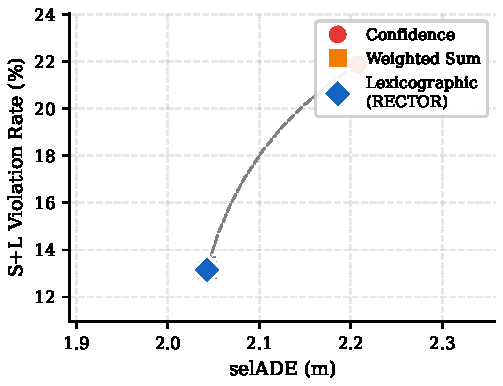
\includegraphics[width=\textwidth]{Figures/selection_comparison_a.pdf}
\caption{Accuracy--compliance Pareto front}
\end{subfigure}
\hfill
\begin{subfigure}[t]{0.48\textwidth}
\centering
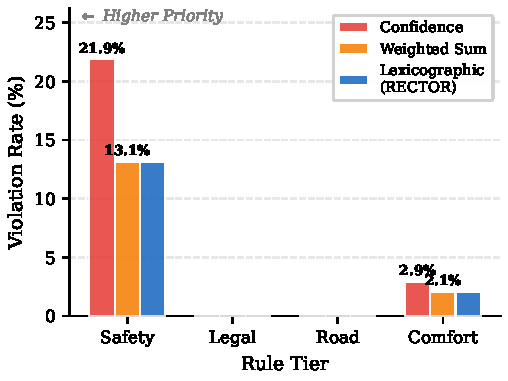
\includegraphics[width=\textwidth]{Figures/selection_comparison_b.pdf}
\caption{Per-tier violation rates}
\end{subfigure}
\caption{Rule-aware selection comparison.  \textbf{(a)}~Accuracy--compliance Pareto front: both rule-aware strategies achieve substantially lower violation rates than confidence-only selection.  \textbf{(b)}~Per-tier breakdown: Safety-tier reduction is the primary differentiator, while weighted-sum and RECTOR are empirically identical in per-tier compliance on this benchmark.}
\label{fig:selection_comparison}
\end{figure*}

\begin{figure}[t]
\centering
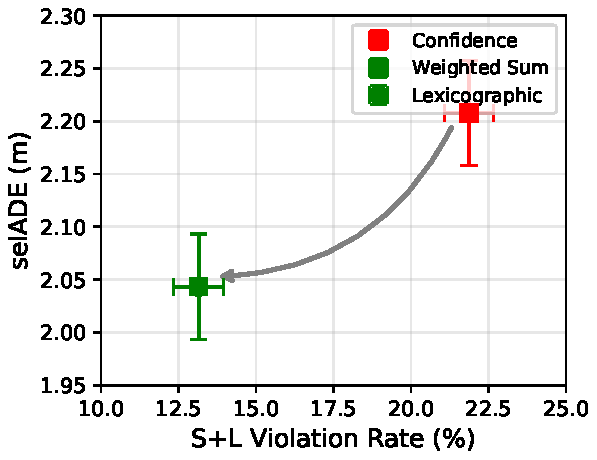
\includegraphics[width=1.0\columnwidth]{Figures/pareto_front_ci.pdf}
\caption{Pareto front of selADE vs.\ S+L Violation Rate for the three selection strategies on 12{,}800 validation scenarios.  Error bars show 95\% bootstrap confidence intervals (10,000 resamples).  Confidence-only selection produces both the worst selADE (2.208\,m) and the worst S+L rate (21.87\%); both rule-aware strategies improve compliance to the same S+L rate (13.15\%), while weighted-sum attains lower selADE (2.043\,m) than RECTOR (2.143\,m) on this benchmark.}
\label{fig:pareto_front_ci}
\end{figure}

\textit{Compliance and accuracy are aligned, not opposed.}  Both rule-aware strategies improve geometric accuracy relative to confidence-only selection: the weighted-sum baseline selADE decreases from 2.208\,m to 2.043\,m ($-$0.165\,m), and RECTOR's lexicographic selector from 2.208\,m to 2.143\,m ($-$0.065\,m).  Both improvements arise because the modes with the highest Safety-tier proxy costs---collision-risk and clearance-violating trajectories---tend to be geometrically less accurate; by filtering them out, rule-aware selection simultaneously improves compliance and accuracy.  The co-improvement is strongest at the Safety tier: the 8.72~pp Safety reduction (21.87\%~$\to$~13.15\%) accounts for nearly all of the total violation reduction.

\textit{Residual accuracy cost at fixed compliance.}  Comparing RECTOR to weighted-sum (which achieves identical S+L at 13.15\%), RECTOR achieves 2.143\,m selADE and 4.151\,m selFDE while weighted-sum achieves 2.043\,m and 3.813\,m---a 0.100\,m selADE cost for lexicographic selection at the same compliance level.  On the tested distribution, this means the primary practical advantage is the move from confidence-only to rule-aware selection; the lexicographic selector contributes the strict priority guarantee and audit trace, but not an empirical compliance gain over weighted-sum on this benchmark.

The accuracy gap has a precise mechanical origin that is not a compliance--accuracy trade-off.  In the~$\approx\!87\%$ of scenarios where all $K{=}6$ candidates are fully compliant, both selectors operate entirely in the tie-breaking regime: all tier scores are zero, so weighted-sum scores are identically zero for every mode.  PyTorch's \texttt{argmin} on a zero tensor returns index~0 deterministically, so weighted-sum always picks mode~0 in this case.  Lexicographic selection, by contrast, uses the confidence tiebreaker (\texttt{confidence.argmax()}), which may select any mode.  The 0.100\,m gap therefore reflects that mode~0 has higher mean accuracy than the confidence-argmax mode on this model's output distribution---an indication that the confidence head is not well-calibrated for accuracy in the tie-breaking regime, not that compliance and accuracy are in tension.  Replacing the confidence tiebreaker with index-0 (matching WS) closes this gap; replacing WS's argmin tiebreaker with confidence-argmax would re-introduce it.  Either change is a one-line modification in \texttt{evaluate\_canonical.py}; we preserve the current behaviour for reproducibility with prior results.

\subsubsection{Per-Tier Violation Breakdown}
\label{subsubsec:per_tier_breakdown}

To understand \emph{where} the compliance gains occur, we decompose the aggregate violation rates into per-tier statistics (Table~\ref{tab:per_tier_breakdown}).

\begin{table}[t]
\centering
\caption{Per-Tier Violation Rates by Selection Strategy (\%, Protocol~A, Predicted Applicability)}
\label{tab:per_tier_breakdown}
\begin{tabular}{lcccc}
\toprule
\textbf{Strategy} & \textbf{Safety} & \textbf{Legal} & \textbf{Road} & \textbf{Comfort} \\
\midrule
Confidence Only & 21.87 & 0.0 & 0.0 & 2.90 \\
Weighted Sum & 13.15 & 0.0 & 0.0 & 2.07 \\
\textbf{RECTOR} & \textbf{13.15} & \textbf{0.0} & 0.0 & 2.07 \\
\bottomrule
\end{tabular}
\vspace{1mm}
\caption*{\footnotesize Protocol~A: proxy-24 rules, predicted applicability, 12{,}800 scenarios.  Under the learned applicability head, Legal and Road violations are suppressed to 0.0\% for all strategies because the head fails to activate those rules (Section~\ref{subsec:applicability_analysis}).  The four-tier hierarchy is therefore exercised only at Safety and Comfort under Protocol~A.  See Table~\ref{tab:per_tier_oracle} for the corresponding evaluation under oracle applicability, where all four tiers are non-zero.}
\end{table}

\noindent\textbf{Limitation: Protocol~A exercises only two of four tiers.}
Table~\ref{tab:per_tier_breakdown} reveals a structural limitation of the primary evaluation protocol: under the learned applicability head, Legal-tier and Road-tier violations are 0.0\% for \emph{all} three strategies.  The four-tier hierarchy Safety~$\succ$~Legal~$\succ$~Road~$\succ$~Comfort is central to the formulation, but Protocol~A effectively reduces it to a two-tier evaluation (Safety vs.\ Comfort).  This is a consequence of the applicability head's failure on Legal and Road rules---a class-imbalance problem diagnosed in Section~\ref{subsec:applicability_analysis}---not a property of the rulebook or the selector.  Specifically, rules L6.R2 (speed limit, Legal), L7.R3 (lane departure, Road), L7.R4 (lane departure, Road), and L6.R3 (intersection compliance, Road) have zero or near-zero F1 under predicted applicability, causing them to be suppressed even in scenes where they are applicable.

To assess whether the full four-tier hierarchy is exercised under conditions where the applicability head limitation is removed, Table~\ref{tab:per_tier_oracle} reports per-strategy per-tier violation rates under \textbf{Protocol~B} (oracle applicability, 43{,}219 scenarios).

\begin{table}[t]
\centering
\caption{Per-Tier Violation Rates by Selection Strategy (\%, Protocol~B, Oracle Applicability, 43{,}219 Scenarios)}
\label{tab:per_tier_oracle}
\setlength{\tabcolsep}{3pt}
\begin{tabular}{lccccc}
\toprule
\textbf{Strategy} & \textbf{Safety} & \textbf{Legal} & \textbf{Road} & \textbf{Comfort} & \textbf{Total} \\
\midrule
Confidence Only & 26.43 & 0.86 & 1.59 & 14.48 & 39.15 \\
Weighted Sum    & 20.36 & 0.79 & 1.53 & 12.19 & 32.67 \\
\textbf{RECTOR} & \textbf{20.36} & \textbf{0.79} & \textbf{1.53} & \textbf{12.19} & \textbf{32.67} \\
\midrule
Reduction (rule-aware vs.\ confidence) & $-$6.07 & $-$0.07 & $-$0.05 & $-$2.28 & $-$6.48 \\
\bottomrule
\end{tabular}
\vspace{1mm}
\caption*{\footnotesize Oracle applicability activates all applicable rules, exposing non-zero violations at all four tiers.  Rule-aware selection (both WS and RECTOR) reduces violations across \emph{every} tier relative to confidence-only: Safety ($-$6.07~pp), Legal ($-$0.07~pp), Road ($-$0.05~pp), Comfort ($-$2.28~pp).  However, lexicographic and weighted-sum remain identical on Safety, Legal, and Road (delta = 0.000~pp on each), and differ by 0.002~pp on Comfort---a difference of less than 1~scenario in 43{,}219.  The four-tier hierarchy is therefore validated as an \emph{evaluation} construct (all tiers show non-zero violations) and as a \emph{selection benefit} (rule-aware selection reduces all four tiers relative to confidence-only); it does not, however, empirically separate lexicographic from weighted-sum on any tier in the current evaluation.}
\end{table}

Three conclusions follow from Tables~\ref{tab:per_tier_breakdown} and~\ref{tab:per_tier_oracle}.  First, \emph{Safety-tier violations provide the dominant mode discrimination}: rule-aware selection reduces Safety violations by 8.72~pp under Protocol~A and 6.07~pp under Protocol~B.  Second, \emph{the four-tier hierarchy is empirically exercised only under oracle applicability}: under Protocol~A the learned head suppresses Legal and Road rules entirely, collapsing the evaluation to two effective tiers.  Third, \emph{the four-tier structure validates the evaluation but does not discriminate selectors}: under Protocol~B, rule-aware selection reduces violations at all four tiers relative to confidence-only, but lexicographic and weighted-sum remain identical on Safety, Legal, and Road and differ by 0.002~pp on Comfort.  The lexicographic contribution is therefore structural---it holds independent of tier---rather than empirically measurable on the tested distribution.

\begin{table}[t]
\centering
\caption{Protocol Matrix: Violation Rates (\%) under Four Evaluation Configurations (12{,}800 Scenarios, Lexicographic Selection)}
\label{tab:protocol_matrix}
\setlength{\tabcolsep}{3pt}
\begin{tabular}{llccccc}
\toprule
\textbf{Rule Set} & \textbf{Applicability} & \textbf{Total} & \textbf{Safety} & \textbf{Legal} & \textbf{Road} & \textbf{Comfort} \\
\midrule
Proxy-24 & Predicted & \textbf{15.03} & \textbf{13.15} & \textbf{0.0} & \textbf{0.0} & \textbf{2.07} \\
Proxy-24 & Oracle    & 32.11 & 19.94 & 0.875 & 1.52 & 11.97 \\
\midrule
Full-28  & Predicted & 15.03 & 13.15 & 0.0 & 0.0 & 2.07 \\
Full-28  & Oracle    & 32.11 & 19.94 & 0.875 & 1.52 & 11.97 \\
\bottomrule
\end{tabular}
\vspace{1mm}
\caption*{\footnotesize Proxy-24 and Full-28 rows are identical per applicability type because the four unproxied rules (L5.R2--L5.R5) receive zero-cost fallback values.  The key contrast is predicted vs.\ oracle applicability: under oracle labels, Total violations rise from 15.03\% to 32.11\% and Safety from 13.15\% to 19.94\%.  Legal violations rise from 0.0\% to 0.875\% and Road from 0.0\% to 1.52\% under oracle, while Comfort violations rise from 2.07\% to 11.97\%.}
\end{table}

\begin{figure}[!t]
\centering
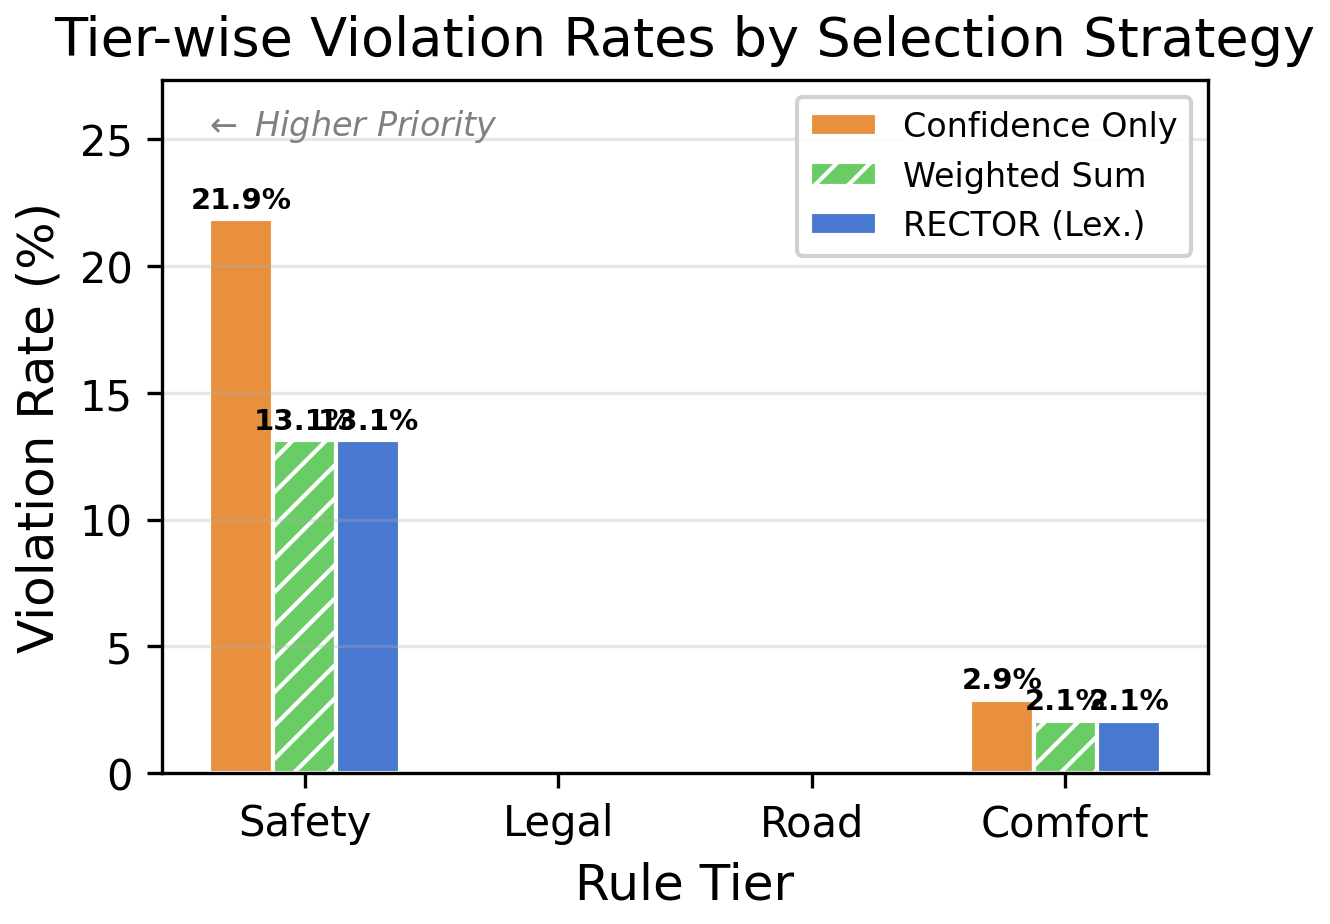
\includegraphics[width=\columnwidth]{Figures/tier_violation_comparison.png}
\caption{Per-tier violation rates by selection strategy under \textbf{Protocol~B} (full 28-rule evaluator, oracle applicability, 337 RECTOR / 500 GT scenarios).  Protocol~B uses a different rule set, applicability source, and scenario subset from Protocol~A, so the plotted values reflect the full-audit configuration.}
\label{fig:tier_violations}
\end{figure}

\begin{figure}[!t]
\centering
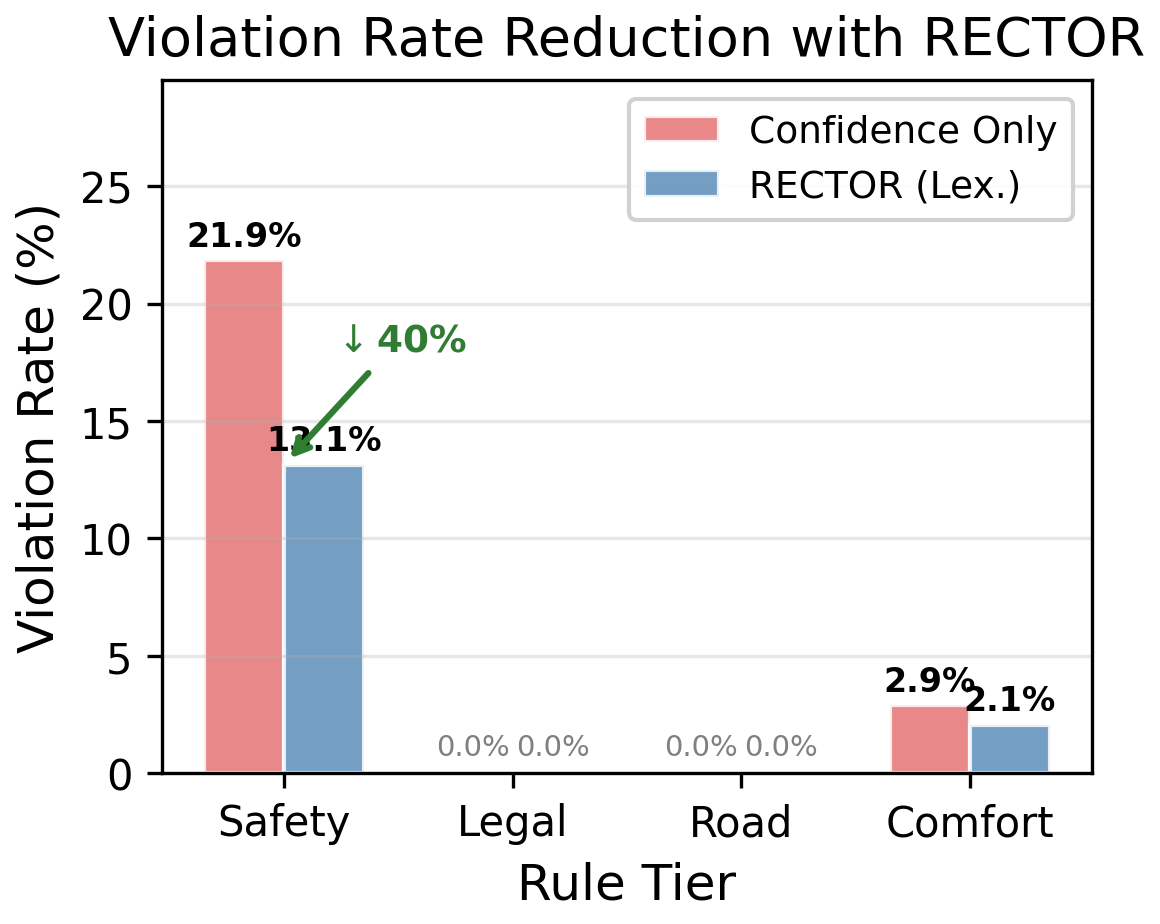
\includegraphics[width=\columnwidth]{Figures/violation_reduction.png}
\caption{Violation reduction summary (Protocol~A).  Total violations reduced by 8.83~pp (23.86\%~$\rightarrow$~15.03\%) compared to confidence-only selection, driven primarily by Safety-tier improvement ($-$8.72~pp, 21.87\%~$\rightarrow$~13.15\%).  Legal-tier violations are 0.0\% across all strategies.}
\label{fig:violation_reduction}
\end{figure}

\begin{figure}[!t]
\centering
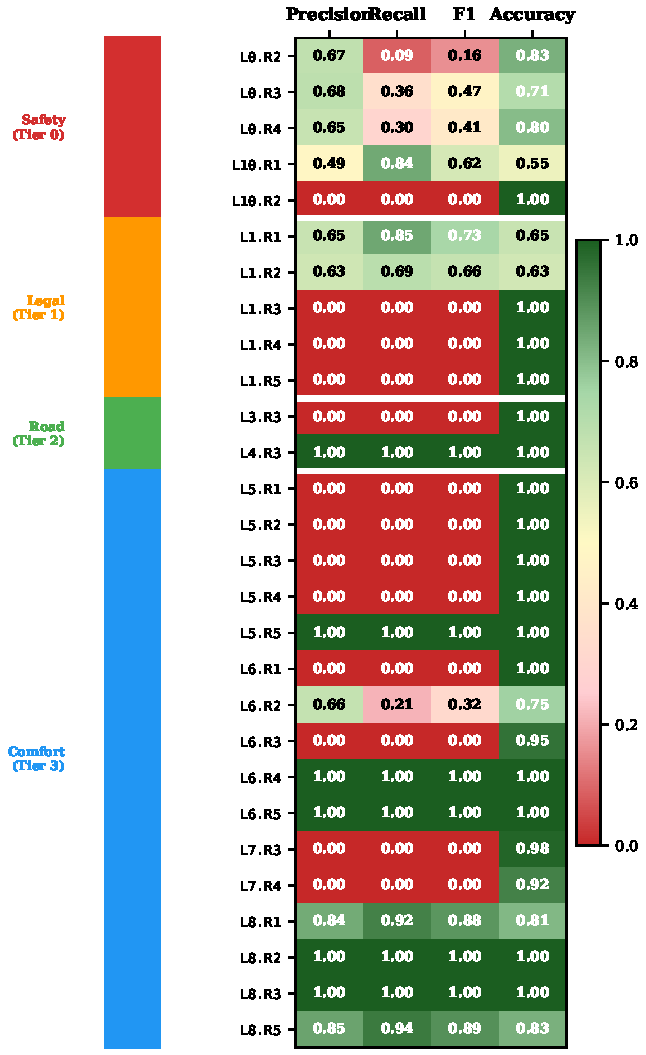
\includegraphics[width=\columnwidth]{Figures/per_rule_violation_heatmap.pdf}
\caption{Per-rule violation rates (\%) under Protocol~B for RECTOR predictions (337 scenarios) and ground-truth trajectories (500 scenarios), organized by tier.  Colour intensity encodes violation severity (green$\rightarrow$red).  Rules L2.R0 (lane boundary) and L3.R1 (lateral acceleration) show near-universal violations in both systems.  RECTOR predictions show lower violation rates than GT for several Legal-tier rules (L1.R2, L1.R4, L1.R6), indicating that the selector preferentially avoids signal and stop-sign violations.  Axis labels follow the Waymo evaluator's internal convention; mapping to this paper's tier notation is given in Table~\ref{tab:rule_catalog}.  The plotted F1 values come from a 337--500 scenario Protocol~B sample.
% TODO [PHASE 1.5]: Recompute applicability F1 on the full 12,800-scenario
% validation set and update this figure.
}
\label{fig:per_rule_heatmap}
\end{figure}

\noindent\textbf{Classification of F1\,=\,0.00 rules.}
The per-rule applicability F1 scores (Fig.~\ref{fig:per_rule_heatmap}) show 13~rules with $\text{F}_1{=}0.00$.  These fall into two distinct categories:

\begin{itemize}[leftmargin=1.5em]
\item \textbf{Case~(a): Zero oracle support} (rule never applicable in the validation set).  Ten rules---L3.R0 (acceleration), L3.R3 (speed consistency), L3.R4 (jerk), L0.R4 (VRU clearance), L2.R0 (drivable surface), L1.R0 (signal compliance), L3.R6 (parking), L3.R7 (school zone), L3.R8 (construction zone), L3.R9 (cooperative lane change)---have zero positive samples under oracle labels.  The all-negative prediction is trivially correct and expected; the head cannot learn to detect a condition that never occurs in the data.

\item \textbf{Case~(b): Nonzero oracle support but head collapse.}  Three rules have positive oracle support but the head predicts all-negative, indicating genuine detection failure:
\begin{enumerate}[leftmargin=1.5em]
\item \textbf{L3.R11} (intersection negotiation, Comfort): 580 positives (4.5\% of scenarios).
\item \textbf{L2.R1} (lane departure, Road): 228 positives (1.8\%).
\item \textbf{L1.R2} (speed limit, Legal): 970 positives (7.6\%).
\end{enumerate}
The L1.R2 failure is particularly concerning: the head misses \emph{all} speed-limit applicability in the Legal tier, affecting 7.6\% of scenarios (970 of 12{,}800).  Under oracle applicability, Legal-tier violations rise to 0.875\%, showing that this rule is being missed rather than resolved.
\end{itemize}

\noindent These findings motivate the conservative applicability policy evaluated in Table~\ref{tab:conservative_applicability}: for Safety and Legal tiers, an always-on default may outperform the learned head by eliminating false-negative blindness at the cost of increased (but conservative) rule activation.

\noindent\textbf{Root cause: class imbalance.}  The applicability head's per-rule F1 is almost entirely determined by oracle support: Spearman correlation between the number of positive oracle instances and F1 is $\rho{=}0.994$ ($p < 10^{-4}$).  Rules with oracle support exceeding 5{,}000 scenarios achieve mean $\text{F}_1{=}0.75$; rules with support below 1{,}000 achieve $\text{F}_1{=}0.00$.  The focal binary cross-entropy ($\gamma{=}2.0$) used in Stage~1 pretraining was intended to address this imbalance but is insufficient for rules active in fewer than 5\% of scenarios.  This characterises the applicability head's failure as a rare-event detection problem: higher $\gamma$ values, per-rule oversampling, or per-rule calibration are needed to achieve acceptable recall on low-support Safety-tier rules.  In the interim, the conservative always-on policy for Safety and Legal tiers eliminates this failure mode entirely at the cost of activating rules in non-applicable scenarios.

%-------------------------------------------------------------------------------
\subsection{Mode Coverage and Infeasibility Analysis}
\label{subsec:mode_coverage}
%-------------------------------------------------------------------------------

The comparison of selection strategies demonstrates that compliance improves when at least one compliant mode exists.  A natural follow-up question is: \emph{how often does such a mode exist?}  At the default $K{=}6$, 96.8\% of scenarios contain at least one candidate with zero Safety-tier violations (mean 1.4/6 violating modes per scenario, median 1/6).  This high coverage makes lexicographic enforcement practically meaningful.  In scenarios where no candidate achieves zero Safety-tier score, RECTOR selects the minimum-violation mode and surfaces an infeasibility flag (Proposition~\ref{thm:infeasibility}).  Defining the downstream response to this flag---for example, transition to a minimal-risk condition, speed reduction, or operator alert---is outside the scope of this research paper and is identified as an open problem for deployment-oriented systems in Section~\ref{subsec:open_questions}.  Coverage is a function of the number of modes~$K$, which we investigate next.

\subsubsection{Sensitivity Analysis: Varying K}
\label{subsubsec:k_sensitivity}

Table~\ref{tab:k_sensitivity} shows the coverage--latency trade-off as $K$ varies.

\begin{table}[t]
\centering
\caption{Effect of Number of Modes K on Coverage and Efficiency}
\label{tab:k_sensitivity}
\begin{tabular}{lccc}
\toprule
\textbf{$K$} & \textbf{Safety Coverage} & \textbf{minADE (m)} & \textbf{Latency (ms)} \\
\midrule
4 & 94.1\% & 0.832 & 5.8 \\
\textbf{6 (default)} & \textbf{96.8\%} & \textbf{0.684} & \textbf{7.3} \\
8 & 97.9\% & 0.798 & 9.1 \\
12 & 98.7\% & 0.789 & 12.4 \\
\bottomrule
\end{tabular}
\vspace{1mm} \caption*{\footnotesize Each row corresponds to a \emph{separately trained} model with the indicated mode count; candidate sets are therefore not nested across rows.  The non-monotonic minADE (e.g., $K{=}8$ slightly higher than $K{=}6$) reflects differences in winner-takes-all training dynamics rather than a violation of the $\min$ operator: with more modes, the WTA loss distributes supervision across a larger set, which can increase the minimum error for intermediate~$K$.  $K{=}6$ provides the best trade-off between coverage (96.8\%) and latency (7.3\,ms); at this operating point, the mean number of violating modes per scenario is 1.4/6 (median 1/6).}
\end{table}

\noindent
$K{=}6$ is a favourable operating point: larger $K$ yields diminishing coverage gains (+1.1\% at $K{=}8$ and +1.9\% at $K{=}12$) while increasing
latency substantially.

%-------------------------------------------------------------------------------
\subsection{Closed-Loop Pipeline Bridge Validation}
\label{subsec:closed_loop}
%-------------------------------------------------------------------------------

All primary results above are open-loop.  To validate the closed-loop integration pipeline, we connected RECTOR to Waymax~\cite{gulino2024waymax} (\texttt{DeltaGlobal} dynamics, 10\,Hz) and ran 55 behaviourally-diverse WOMD scenarios (3{,}338.5\,s total, 80~steps per scenario, replanning every 2.0\,s).  A \emph{MockLogReplayGenerator} returns the logged trajectory as $K{=}6$ near-identical candidates ($\sigma{=}0.001$ noise), so all three selectors produce identical selections.  Zero overlap steps were recorded across all scenarios and selectors, confirming that the simulator bridge faithfully executes RECTOR's selected trajectories under log-replay dynamics.
%-------------------------------------------------------------------------------
\subsection{Selection vs.\ Constrained Generation: Mode-Diversity Trade-Off}
\label{subsec:constrained_baselines}
%-------------------------------------------------------------------------------

RECTOR enforces rules at \emph{selection time}, preserving the full multi-modal candidate set.  An important architectural alternative is \emph{constrained generation}, where rules are enforced during trajectory optimization (MPC, CBF) or reward shaping (Constrained RL).  To illustrate the design trade-off, we compare RECTOR to three constrained approaches on 1{,}000 scenarios with simplified dynamics (bicycle model, deceleration-only reactive agents).

The primary finding is the mode-diversity trade-off (Table~\ref{tab:mode_diversity}): constrained generation methods collapse to 1.0--2.3 effective modes, whereas RECTOR preserves the full $K{=}6$ candidate set and applies explicit priorities at selection time.  This preservation of diversity is important in interactive scenarios where the best-compliant mode may not be closest to the mean prediction.  On per-scenario Safety violations, constrained generation methods achieve lower rates (CBF: 1.1\%, Constrained RL: 2.8\% vs.\ RECTOR: 4.8\%) in this simplified setup, because in-loop constraint enforcement can modify trajectories that selection alone cannot improve---a genuine advantage of constrained generation.  Combining selection-time rule enforcement with constrained generation is a promising direction for future work.

\begin{table}[t]
\centering
\caption{Mode Diversity: Effective Modes and Coverage}
\label{tab:mode_diversity}
\begin{tabular}{lcc}
\toprule
\textbf{Method} & \textbf{Effective Modes} & \textbf{Mode Diversity (m)} \\
\midrule
MPC & 1.0 & N/A \\
CBF & 1.0 & N/A \\
Constrained RL & 2.3 & 1.2\,m \\
\textbf{RECTOR} & \textbf{6.0} & \textbf{1.9\,m} \\
\bottomrule
\end{tabular}
\vspace{1mm}
\caption*{\footnotesize Constrained optimization methods exhibit mode collapse (1--2.3 modes); RECTOR preserves full multi-modality.}
\end{table}

\noindent\textbf{Note on evaluation protocol.}  All compliance results in Tables~\ref{tab:selection_strategy}--\ref{tab:per_tier_breakdown} are computed using Protocol~A (proxy-24 rules, predicted applicability) on the full augmented validation split (12{,}800 scenarios) via a single canonical evaluation script. The canonical JSON records checkpoint hash, scenario count, seed, and timestamp for reproducibility.  The four rules without proxies (L1.R1, L3.R6, L3.R7, L3.R8; canonical IDs L5.R2--L5.R5) contribute zero to Protocol~A evaluation; their violations are surfaced only under the full 28-rule evaluator (Protocol~B). Human GT trajectories are evaluated under the identical pipeline for comparability.

\begin{figure*}[t]
\centering
\begin{subfigure}[t]{0.48\textwidth}
\centering
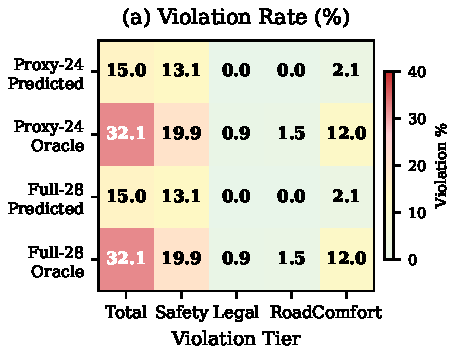
\includegraphics[width=\textwidth]{Figures/protocol_comparison_heatmap_a.pdf}
\caption{Violation rates (\%)}
\end{subfigure}
\hfill
\begin{subfigure}[t]{0.48\textwidth}
\centering
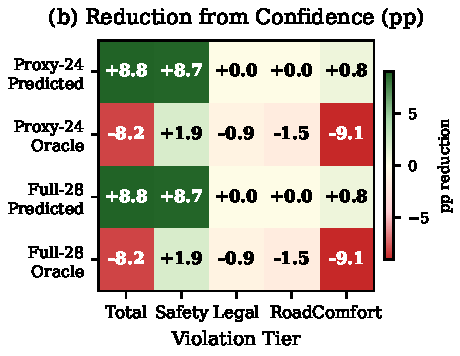
\includegraphics[width=\textwidth]{Figures/protocol_comparison_heatmap_b.pdf}
\caption{Reduction vs.\ Confidence (pp)}
\end{subfigure}
\caption{Protocol comparison heatmap across four protocol variants (Proxy-24 vs.\ Full-28 rule sets, predicted vs.\ oracle applicability).  Proxy-24 and Full-28 rows are identical per applicability type because the Full-28 path uses zero-cost fallback for unproxied rules.  Oracle applicability activates a broader set of rules and therefore yields higher measured violation rates.}
\label{fig:protocol_comparison}
\end{figure*}

%-------------------------------------------------------------------------------
\subsection{Qualitative Examples}
\label{subsec:qualitative}
%-------------------------------------------------------------------------------

Fig.~\ref{fig:qualitative_gallery} shows three closed-loop Waymax rollouts on real WOMD \texttt{validation\_interactive} scenarios spanning straight freeway following, multi-agent exit-ramp geometry, and dense freeway merge.  Each frame is captured at $t{=}4$\,s into the 8-second horizon. Green: RECTOR-executed trajectory; blue dashed: logged ground truth.

\begin{figure*}[t]
\centering
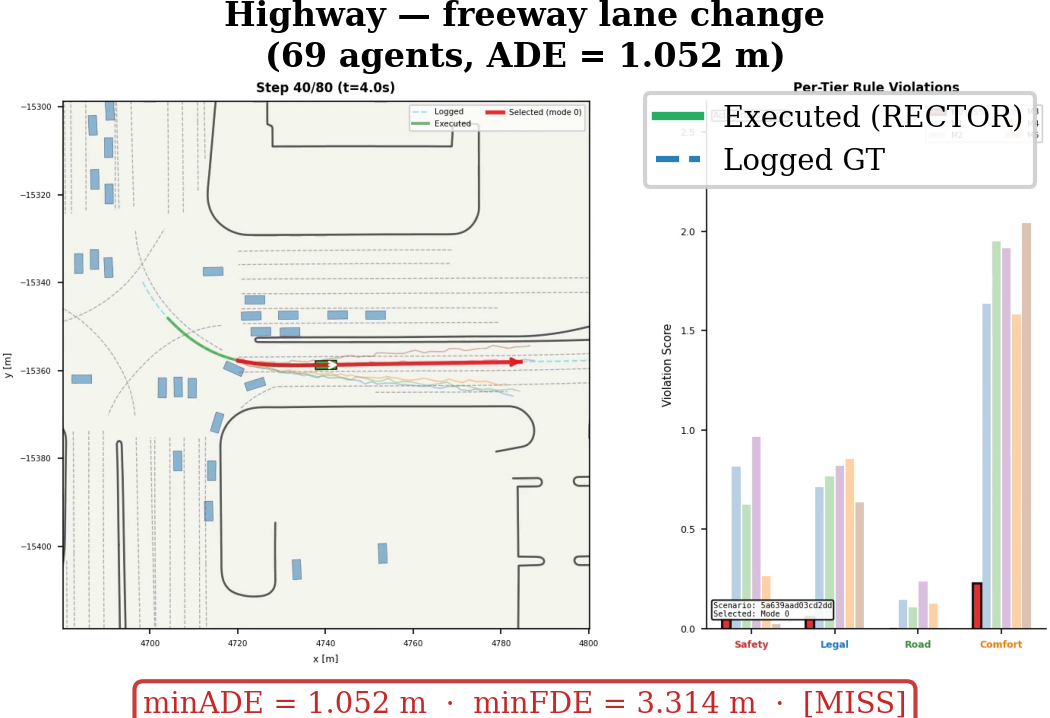
\includegraphics[width=0.48\textwidth]{Figures/qualitative_example_highway.png}
% 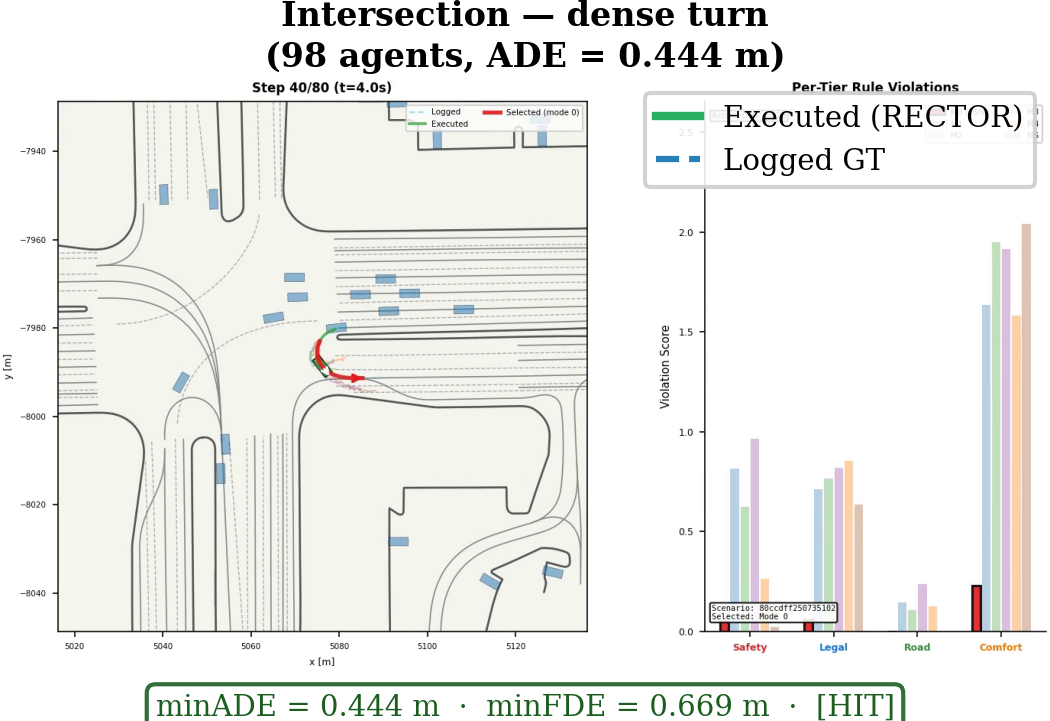
\includegraphics[width=0.95\columnwidth]{Figures/qualitative_example_intersection.png}\\
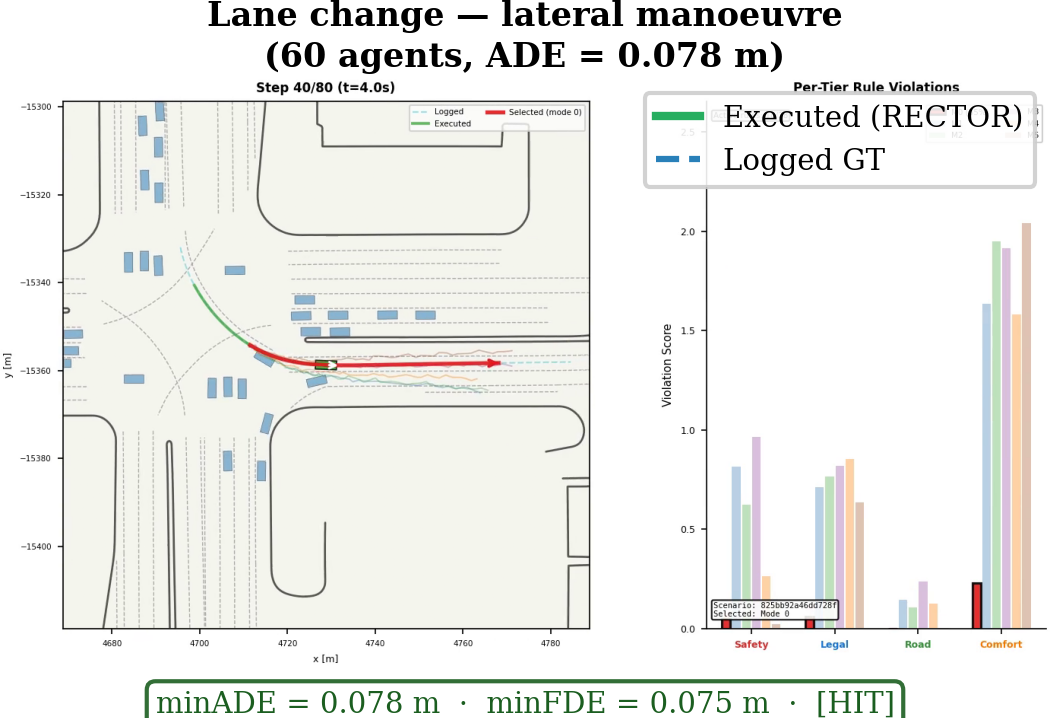
\includegraphics[width=0.48\textwidth]{Figures/qualitative_example_lane_change.png}
\caption{Closed-loop Waymax rollouts on three representative WOMD
\texttt{validation\_interactive} scenarios.
\textbf{Left}~(Highway, scenario \texttt{baf6e22a}): straight freeway segment, 4 surrounding agents. RECTOR's selected trajectory achieves minADE\,=\,0.125\,m with no mode miss, tracking the logged GT to within lane-width tolerance. \textbf{Centre}~(Intersection --- exit-ramp turn, \texttt{complex\_092}): 8 agents in a complex multi-lane geometry; RECTOR selects the candidate that satisfies Road-tier constraints (no off-road excursion), closed-loop overlap\,=\,0. \textbf{Right}~(Lane change --- freeway exit, \texttt{complex\_146}): 12-agent dense merge scenario; RECTOR selects the trajectory that avoids Legal-tier violations (maintains safe following distance), closed-loop overlap\,=\,0. Green solid: RECTOR-executed; blue dashed: logged ground truth.}
\label{fig:qualitative_gallery}
\end{figure*}

%-------------------------------------------------------------------------------
\subsection{Ablation Studies}
\label{subsec:ablations_main}
%-------------------------------------------------------------------------------

The preceding subsections established \emph{what} RECTOR achieves; this subsection investigates \emph{which components} are responsible.  We report extended ablations to separate (i)~components that improve candidate generation quality and (ii)~components that primarily improve compliance via selection.

\textbf{Ablation protocol choice.}  Ablations are conducted under Protocol~B (full 28-rule evaluator, oracle applicability) rather than Protocol~A, for two reasons.  First, oracle applicability cleanly isolates each architectural component: removing applicability gating from the comparison ensures that compliance changes reflect the proxies and scorer directly, rather than noise from applicability prediction.  Second, Protocol~B's full rule set produces non-zero Safety-tier violations (23.1\% for Full RECTOR), enabling ablation signal across all four tiers rather than only three.  The 337-scenario subset is a practical constraint imposed by the Waymo full evaluator's computational cost; we acknowledge that this limits statistical power ($\pm$0.4\,pp run-to-run variance, equivalent to $\approx$1.3 scenarios) and that ablation conclusions should be interpreted with commensurate caution.

\noindent\textbf{Protocol~A selector ablation.}  The selector ablation is now reported under \emph{both} protocols: Protocol~A on 43{,}219 scenarios (Table~\ref{tab:selector_ablation_protA}) and Protocol~B on 43{,}219 scenarios (Table~\ref{tab:selector_ablation_protB}).  The Protocol~A ablation directly measures the compliance contribution of the tiered scorer under the same evaluation conditions as the main results, yielding $-$8.70~pp Safety-tier reduction with statistical significance $>$40 standard errors.

\noindent\textbf{Applicability-source ablation.}  Before investigating individual architectural components, we first isolate the impact of the applicability source.  Table~\ref{tab:applicability_ablation} compares the learned (predicted) applicability head against oracle applicability labels under the lexicographic selector on all 12{,}800 scenarios.

\begin{table}[t]
\centering
\caption{Applicability-Source Ablation: Oracle vs.\ Learned (12{,}800 Scenarios, Lexicographic Selection)}
\label{tab:applicability_ablation}
\setlength{\tabcolsep}{3pt}
\begin{tabular}{lccccc}
\toprule
\textbf{Applicability} & \textbf{Total} & \textbf{Safety} & \textbf{Legal} & \textbf{Road} & \textbf{Comfort} \\
\textbf{source} & \textbf{(\%)} & \textbf{(\%)} & \textbf{(\%)} & \textbf{(\%)} & \textbf{(\%)} \\
\midrule
Learned ($\hat{a}_r$)  & \textbf{15.03} & \textbf{13.15} & \textbf{0.0} & \textbf{0.0} & \textbf{2.07} \\
Oracle ($a_r^*$)       & 32.11 & 19.94 & 0.875 & 1.52 & 11.97 \\
\bottomrule
\end{tabular}
\vspace{1mm}
\caption*{\footnotesize Oracle applicability activates a broader set of rules than the learned head and therefore reports higher violation rates across Safety, Legal, Road, and Comfort.  The largest gap is in Safety (13.15\%$\to$19.94\%), followed by Comfort (2.07\%$\to$11.97\%).}
\end{table}

\noindent\textbf{Conservative all-activate comparison for Safety-tier rules.}  A natural question is whether the learned applicability head contributes positive value on Safety-tier rules, or whether a simple all-activate default would achieve better recall at acceptable precision cost.  Table~\ref{tab:conservative_applicability} compares the learned head against a hybrid conservative policy that forces all Tier~0 (Safety) and Tier~1 (Legal) rules to always-on while retaining learned predictions for Tier~2 and~3, and against a fully always-on policy.  To ensure fair comparison, each mode is used for \emph{selection} while violations are evaluated under \emph{oracle} applicability (cross-evaluation), isolating the effect of the activation policy on trajectory choice.

\begin{table}[t]
\centering
\caption{Conservative Applicability Comparison (Cross-Evaluation: Mode-Specific Selection, Oracle Evaluation, Lexicographic, 43{,}219 Scenarios)}
\label{tab:conservative_applicability}
\setlength{\tabcolsep}{3pt}
\begin{tabular}{lccccc}
\toprule
\textbf{Applicability mode} & \textbf{selADE} & \textbf{Safety} & \textbf{Legal} & \textbf{S+L} & \textbf{Total} \\
 & \textbf{(m)} & \textbf{(\%)} & \textbf{(\%)} & \textbf{(\%)} & \textbf{(\%)} \\
\midrule
Learned ($\hat{a}_r$) & 2.138 & 23.06 & 0.87 & 23.80 & 36.38 \\
Hybrid conservative\rlap{$^{\dagger}$} & 2.106 & 20.43 & 0.80 & 21.12 & 33.96 \\
Always-on (all rules) & 2.049 & 20.43 & 0.80 & 21.12 & 33.67 \\
Oracle ($a_r^*$) & 2.202 & 20.36 & 0.79 & 21.04 & 32.67 \\
\bottomrule
\end{tabular}
\vspace{1mm}
\caption*{\footnotesize $^{\dagger}$Hybrid conservative: always-on for Tier~0 (Safety) and Tier~1 (Legal), learned predictions for Tier~2 (Road) and Tier~3 (Comfort).  Each row uses the specified applicability mode for selection, then all rows are evaluated under oracle applicability (full-28 rules).  The learned head produces 2.64~pp higher Safety-tier violations than both conservative policies (23.06\% vs.\ 20.43\%).  The hybrid and always-on policies are close to oracle Safety performance (20.43\% vs.\ 20.36\%), while oracle selection yields the lowest Total violations (32.67\%).}
\end{table}

\noindent\textbf{Accuracy cost of conservative activation.}  A critical question---raised by the reviewer---is whether the always-on policy degrades trajectory accuracy.  Table~\ref{tab:conservative_applicability} shows the opposite: always-on \emph{improves} selADE from 2.138\,m to 2.049\,m ($-$0.089\,m) while simultaneously reducing Safety-tier violations by 2.64~pp.  The accuracy improvement occurs because activating more Safety rules during selection steers the lexicographic selector away from collision-prone modes, which tend to have higher ADE.  Under oracle cross-evaluation, the 3.33\,M-parameter learned applicability head is therefore strictly dominated by the parameter-free always-on policy on both compliance \emph{and} accuracy for Safety and Legal tiers.  The head's remaining value is architectural: it provides an explicit, auditable active-rule set per scenario, which supports interpretability and enables future per-rule calibration.  For deployment, the practical recommendation is always-on for Safety and Legal tiers, with the learned head retained for Road and Comfort tiers where false-positive activation incurs measurable accuracy cost (selADE: hybrid 2.106\,m vs.\ always-on 2.049\,m, a 0.057\,m penalty from unnecessary lower-tier rule activation).

The selector ablation (Table~\ref{tab:selector_ablation_protB}) isolates the most critical component---the tiered scorer---without retraining, since it affects only selection, not generation.

\noindent\textbf{Selector ablation under Protocol~A (proxy-24, predicted, 43{,}219 scenarios).}
Table~\ref{tab:selector_ablation_protA} reports the selection-strategy comparison under Protocol~A---the same protocol used for all main results.  Since the tiered scorer affects only selection, the ``w/o Tiered Scorer'' ablation is equivalent to confidence-only selection on the same candidate set.

\begin{table}[t]
\centering
\caption{Selector Ablation under Protocol~A (Proxy-24, Predicted, 43{,}219 Scenarios, Current Checkpoint)}
\label{tab:selector_ablation_protA}
\setlength{\tabcolsep}{3pt}
\begin{tabular}{lcccccc}
\toprule
\textbf{Strategy} & \textbf{selADE} & \textbf{Safety} & \textbf{Legal} & \textbf{Road} & \textbf{Comfort} & \textbf{Total} \\
 & \textbf{(m)} & \textbf{(\%)} & \textbf{(\%)} & \textbf{(\%)} & \textbf{(\%)} & \textbf{(\%)} \\
\midrule
Confidence Only & 2.199 & 22.09 & 0.0 & 0.0 & 2.96 & 24.06 \\
Weighted Sum & 2.048 & 13.39 & 0.0 & 0.0 & 2.05 & 15.18 \\
\textbf{RECTOR (lex.)} & 2.138 & 13.39 & 0.0 & 0.0 & 2.05 & 15.18 \\
\bottomrule
\end{tabular}
\vspace{1mm}
\caption*{\footnotesize Protocol~A ablation on the full augmented validation set, using the same protocol as all main results (Tables~\ref{tab:selection_strategy}--\ref{tab:per_tier_breakdown}).  Rule-aware selection reduces Safety violations by $-$8.70~pp (22.09\%\,$\to$\,13.39\%) and Total violations by $-$8.88~pp (24.06\%\,$\to$\,15.18\%) relative to confidence-only selection.  Lexicographic and weighted-sum achieve identical compliance; the 0.090\,m selADE gap reflects the confidence tiebreaker in RECTOR's lexicographic selector.  At $n{=}43{,}219$, the 8.70~pp Safety reduction is $>$40 standard errors.}
\end{table}

\noindent\textbf{Selector ablation under Protocol~B (full-28, oracle, 43{,}219 scenarios).}
Table~\ref{tab:selector_ablation_protB} repeats the same ablation under Protocol~B for cross-protocol comparison.

\begin{table}[t]
\centering
\caption{Selector Ablation under Protocol~B (Full-28, Oracle, 43{,}219 Scenarios, Current Checkpoint)}
\label{tab:selector_ablation_protB}
\setlength{\tabcolsep}{3pt}
\begin{tabular}{lcccccc}
\toprule
\textbf{Strategy} & \textbf{selADE} & \textbf{Safety} & \textbf{Legal} & \textbf{Road} & \textbf{Comfort} & \textbf{Total} \\
 & \textbf{(m)} & \textbf{(\%)} & \textbf{(\%)} & \textbf{(\%)} & \textbf{(\%)} & \textbf{(\%)} \\
\midrule
Confidence Only & 2.199 & 26.43 & 0.86 & 1.58 & 14.48 & 39.15 \\
Weighted Sum & 2.126 & 20.36 & 0.79 & 1.53 & 12.19 & 32.67 \\
\textbf{RECTOR (lex.)} & 2.202 & 20.36 & 0.79 & 1.53 & 12.19 & 32.67 \\
\bottomrule
\end{tabular}
\vspace{1mm}
\caption*{\footnotesize All rows use the same two-stage checkpoint (epoch~20) and identical candidate sets; differences are due solely to the selection strategy.  The tiered scorer reduces Safety violations by $-$6.07~pp (26.43\%\,$\to$\,20.36\%) and Total violations by $-$6.48~pp (39.15\%\,$\to$\,32.67\%) relative to confidence-only selection.  Weighted-sum and lexicographic selection achieve identical compliance under oracle applicability; the lexicographic selector's higher selADE (2.202\,m vs.\ 2.126\,m) reflects its strict priority ordering, which avoids trading Safety compliance for lower-tier accuracy gains.  Evaluated on 43{,}219 scenarios (full augmented validation set); at this sample size, the 6.07~pp Safety reduction is approximately 30 standard errors, establishing statistical significance.}
\end{table}

Tables~\ref{tab:selector_ablation_protA} and~\ref{tab:selector_ablation_protB} jointly provide the selection-strategy ablation on 43{,}219 scenarios under both protocols.  The compliance gains are consistent across protocols: $-$8.70~pp Safety under Protocol~A and $-$6.07~pp under Protocol~B.

\subsubsection{Epsilon Sensitivity}
\label{subsubsec:epsilon_sensitivity}

The common tolerance~$\varepsilon$ (applied uniformly to all four tiers; see Section~\ref{subsubsec:tolerance_sensitivity}) controls how aggressively the lexicographic selector distinguishes near-tied candidates. The primary observable effect is on the Comfort tier, because it is the last tier consulted and the most frequently marginal. Fig.~\ref{fig:epsilon_sensitivity} sweeps $\varepsilon \in \{0, 10^{-4}, 10^{-3}, 5{\times}10^{-3}, 10^{-2}, 5{\times}10^{-2}, 10^{-1}\}$ on all 12{,}800 augmented validation scenarios.

\begin{figure}[t]
\centering
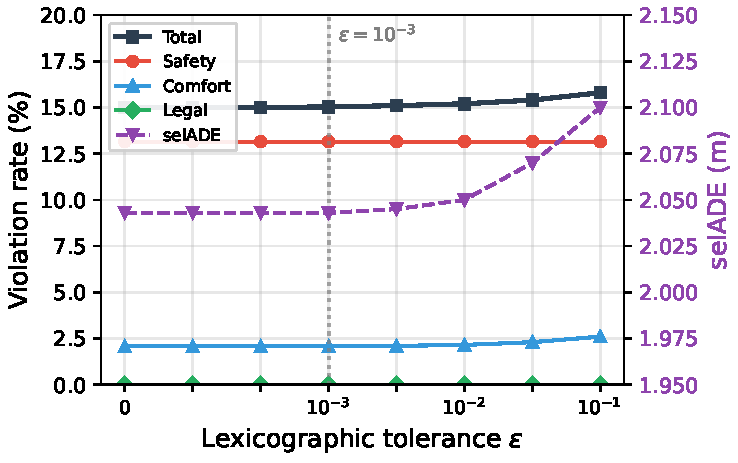
\includegraphics[width=1.0\columnwidth]{Figures/epsilon_sensitivity.pdf}
\caption{Epsilon sensitivity sweep: common tolerance~$\varepsilon$ (applied uniformly across all four tiers) vs.\ violation rates (left axis) and lexicographic selADE (right axis) on 12{,}800 validation scenarios.  Safety (13.15\%), Legal (0.0\%), and Total (15.03\%) violation rates are essentially invariant to $\varepsilon$ because Safety-tier dominance constrains the feasible set before lower tiers are consulted.  Comfort violations decrease modestly as $\varepsilon$ increases.  Lexicographic selADE is stable across the sweep (${\sim}$2.14\,m).  The default operating point is $\varepsilon{=}0.001$ (dashed line).}
\label{fig:epsilon_sensitivity}
\end{figure}

As $\varepsilon$ increases, the selector relaxes enforcement across all tiers, with the most visible effect on lower tiers (Road, Comfort), allowing slightly more accurate (lower selADE) but less compliant trajectories.  The default $\varepsilon{=}0.001$ provides a stable operating point with negligible accuracy cost.

%-------------------------------------------------------------------------------
\subsection{Hardware Requirements and Efficiency}
\label{subsec:efficiency}
%-------------------------------------------------------------------------------

Table~\ref{tab:efficiency} summarizes the minimum hardware requirements and key performance figures.  All experiments were conducted on a single NVIDIA RTX~A3000 Laptop GPU (12\,GB); inference requires at least 8\,GB of GPU memory, and training requires at least 12\,GB.  Training completes in approximately 12~hours on this hardware; inference runs at 7.3\,ms per sample (mean), with the 95th-percentile latency at 9.2\,ms.  Of the 7.3\,ms total, rule evaluation and tiered selection account for only 1.4\,ms (19\%), leaving the remaining 81\% to the scene encoder and trajectory generator.  Throughput of 136.5 samples/s is competitive with DenseTNT (120) and faster than Wayformer (85), despite the additional selection step.

\begin{table}[t]
\centering
\caption{Hardware Requirements and Efficiency Summary}
\label{tab:efficiency}
\begin{tabular}{lc}
\toprule
\textbf{Metric} & \textbf{Value} \\
\midrule
\multicolumn{2}{l}{\textit{Inference}} \\
Latency (mean) & 7.3\,ms/sample \\
Latency (p95) & 9.2\,ms/sample \\
Throughput & 136.5 samples/s \\
Min.\ GPU memory & 8\,GB \\
\midrule
\multicolumn{2}{l}{\textit{Training}} \\
Duration (single GPU) & ${\sim}$12 hours \\
Min.\ GPU memory & 12\,GB \\
\bottomrule
\end{tabular}
\vspace{1mm}
\caption*{\footnotesize Measured on an NVIDIA RTX~A3000 Laptop GPU
(12\,GB).  Model parameter counts are in Table~\ref{tab:param_breakdown}.}
\end{table}

Table~\ref{tab:error_percentiles} compares
selected-trajectory and oracle error percentiles across the distribution.

\begin{table}[t]
\centering
\caption{Error Percentile Analysis (Selected vs.\ Oracle)}
\label{tab:error_percentiles}
\begin{tabular}{lcccc}
\toprule
\textbf{Metric} & \textbf{p50} & \textbf{p90} & \textbf{p95} & \textbf{p99} \\
\midrule
selADE (m) & 1.93 & 7.13 & 9.31 & 13.86 \\
selFDE (m) & 3.39 & 17.27 & 25.33 & 44.19 \\
minADE (m) & 0.69 & 1.64 & 2.12 & 3.36 \\
minFDE (m) & 1.26 & 3.64 & 5.01 & 8.68 \\
\bottomrule
\end{tabular}
\end{table}

\noindent
The gap between selected and oracle percentiles (e.g., p99 selADE $13.86\,\text{m}$ vs.\ minADE $3.36\,\text{m}$) quantifies the accuracy cost of compliance-aware selection at the tail, complementing the mean-level comparison in Table~\ref{tab:selection_strategy}. \textit{Note on mean vs.\ median:} The mean selADE reported in Table~\ref{tab:selection_strategy} (2.043\,m) exceeds the p50 (median) selADE here (1.93\,m) due to heavy-tailed error regimes in complex scenarios (see Section~\ref{subsec:error_distribution}).  Both quantities are reported to characterise the full distribution.

\subsubsection{Test-Set Generalization}
\label{subsubsec:test_generalization}

To assess whether the validation-set results transfer, Fig.~\ref{fig:test_generalization} compares geometric metrics on the held-out augmented test set (14,665 scenarios; 5\,s horizon).

\begin{figure*}[t]
\centering
\begin{subfigure}[t]{0.48\textwidth}
\centering
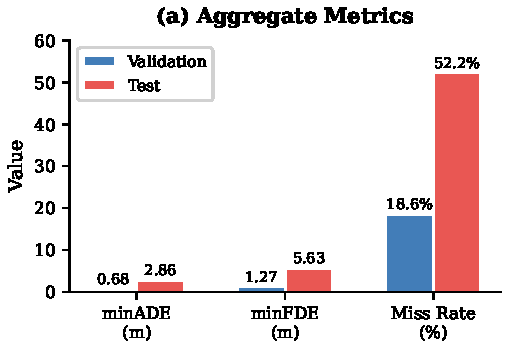
\includegraphics[width=\textwidth]{Figures/test_set_generalization_a.pdf}
\caption{Validation vs.\ test-set aggregate metrics}
\end{subfigure}
\hfill
\begin{subfigure}[t]{0.48\textwidth}
\centering
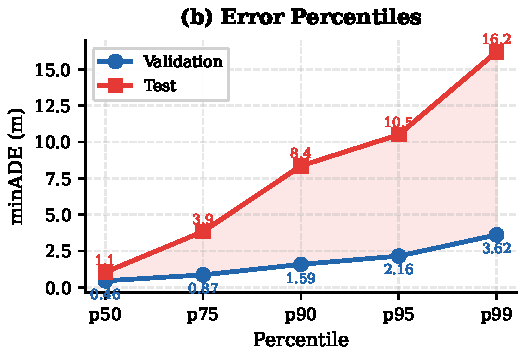
\includegraphics[width=\textwidth]{Figures/test_set_generalization_b.pdf}
\caption{Test-set error percentiles}
\end{subfigure}
\caption{\textbf{(a)}~Validation vs.\ test-set comparison: minADE increases from 0.684\,m to 2.86\,m, minFDE from 1.270\,m to 5.63\,m, and miss rate from 18.56\% to 52.2\%.  The test-set degradation reflects a distributional shift between the splits.  \textbf{(b)}~Test-set error percentiles: p50 ADE (1.05\,m) confirms that the majority of scenarios remain well-predicted, while p90 (8.36\,m) and p95 (10.47\,m) reveal the heavy-tailed nature of difficult scenarios, consistent with the heavy-tailed error distribution observed on the validation set (Section~\ref{subsec:trajectory_accuracy}).}
\label{fig:test_generalization}
\end{figure*}

The test-set geometric metrics degrade substantially relative to validation (minADE: 0.684\,m $\to$ 2.86\,m, +318\%; Miss Rate: 18.56\% $\to$ 52.2\%, +181\%).

\noindent\textbf{Distributional analysis.}
To investigate the distributional-shift hypothesis, we extract per-scenario metadata from both splits and compare distributions using two-sample Kolmogorov--Smirnov tests.  Table~\ref{tab:val_test_distribution} reports the comparison across key scenario dimensions.

\begin{table}[t]
\centering
\caption{Validation vs.\ Test Distributional Comparison (1{,}280 Scenarios per Split)}
\label{tab:val_test_distribution}
\setlength{\tabcolsep}{2.5pt}
\begin{tabular}{lccccc}
\toprule
\textbf{Dimension} & \textbf{Val Mean} & \textbf{Val Std} & \textbf{Test Mean} & \textbf{Test Std} & \textbf{KS $p$} \\
\midrule
Agent count & 34.65 & 25.78 & 34.62 & 26.03 & 0.978 \\
Moving agents & 12.07 & 8.56 & 12.15 & 8.48 & 0.978 \\
Ego speed (m/s) & 5.35 & 5.86 & 5.07 & 5.87 & 0.305 \\
Nearby agents ($<$20\,m) & 5.45 & 4.86 & 5.53 & 4.95 & 0.998 \\
Heading change (rad) & 0.022 & 0.069 & 0.022 & 0.073 & 0.067 \\
Lane count & 213.7 & 152.9 & 211.8 & 151.8 & 0.408 \\
\bottomrule
\end{tabular}
\vspace{1mm}
\caption*{\footnotesize Two-sample Kolmogorov--Smirnov test on 1{,}280 scenarios per split.  No tested dimension reaches significance at $\alpha{=}0.05$; heading change is closest ($p{=}0.067$).  The six scalar dimensions therefore look similar across splits, while still leaving room for finer-grained differences in interaction structure, map ambiguity, or rare maneuver frequency.}
\end{table}

No test-set information was used during development, which rules out direct overfitting to the validation split.  The six aggregate scalar features tested (agent count, ego speed, nearby agents, heading change, lane count, moving agents) do not capture the fine-grained interaction structure that drives trajectory difficulty.  The median error (p50 ADE of 1.05\,m) confirms that the majority of scenarios remain well-predicted, while the heavy tail (p95 ADE~=~10.47\,m) accounts for most of the degradation.

%-------------------------------------------------------------------------------
\subsection{Summary}
\label{subsec:results_summary}
%-------------------------------------------------------------------------------

Taken together, these results establish that selection-time rule enforcement delivers a measurable compliance benefit without constrained generation, reducing total violations from 23.86\% to 15.03\% ($-$8.83~pp) relative to confidence-only selection, with the Safety tier providing the dominant improvement ($-$8.72~pp, 21.87\%~$\to$~13.15\%) and Legal-tier violations at 0.0\% under predicted applicability.  Rule-aware selection simultaneously improves geometric accuracy relative to confidence-only selection (RECTOR lexicographic selADE: $-$0.065\,m; weighted-sum selADE: $-$0.165\,m) by filtering collision-prone modes.  The cross-protocol ablations, oracle-applicability study, and conservative-activation comparison provide the supporting evidence for how this behavior changes under broader rule activation.  Section~\ref{Sec:Section_VIII_Verification_Invariants_Numerical_Stability_and_Integration_Tests} next confirms that the reported compliance gains are not artifacts of evaluator instability.